\documentclass[12pt,a4paper]{article}
\usepackage[utf8]{inputenc}
\usepackage{amsmath}
\usepackage{amsfonts}
\usepackage{amssymb}
\usepackage{graphicx}
\usepackage{float}
\usepackage[table, svgnames, dvipsnames]{xcolor}
\usepackage{booktabs}
\usepackage{graphicx}
\usepackage{float}
\usepackage{ subcaption }
\usepackage{algorithm}
\usepackage{algorithmic}
\graphicspath{ {../images/} }
\author{Alessio Ragno}
\title{Reinforcement Learning Project Report}
\date{November 2019}

\begin{document}

% \maketitle

\begin{titlepage}
    \begin{center}
        \vspace*{1cm}
        
        \huge
        \textbf{Reinforcement Learning Implementation Project Report}
        
        
        \vspace{1.5cm}
        \LARGE
        Alessio Ragno
        
        \vfill
        
        
\includegraphics[width=0.2\textwidth]{sapienza_logo.png}


        
        \vfill
        
  

        \vspace{0.5cm}
        
        
        \large
        Master's Degree in Artificial Intelligence and Robotics\break\break
        Department of Computer, Control and Management Engineering\break\break
        Sapienza University of Rome\break\break
        December 2019

    \end{center}
\end{titlepage}



\pagebreak
\tableofcontents
\pagebreak

\section{Introduction}

What follows is the report for the Reinforcement Learning Implementation Project of Machine Learning Class at Artificial Intelligence and Robotics Course.

The project consists in the implementation of an assigned Reinfocement Learning algorithm and its evaluation in two different environments.

The assigned algorithm is Trust Region Policy Optimization (TRPO) and it has to be evaluated on the following OpenAI Gym environments:
\begin{itemize}
    \item \textbf{MountainCar-v0} is an environment in which a car has to climb a hill and reach a specific point indicated by a flag. MountainCar-v0 is a continuous state space environment that can be controlled with discrete actions. At each timestep the agent can choose between three actions: pushing the car left, right or not applying any force to the car.
    \item \textbf{Pong-v0} is an environment in which the agent has to play Pong game against a virtual player. The state is the image of the game and the agent acts using the Atari 2600 commands: NOOP, FIRE, RIGHT, LEFT, RIGHTFIRE, LEFTFIRE.
\end{itemize}

\section{Trust Region Policy Optimization}

Trust Region Policy Optimization was published by John Schulman, Sergey Levine, Philipp Moritz, Michael I. Jordan and Pieter Abbeel on April 2017. 
TRPO is an improvement of the vanilla Policy Gradient algorithm implemented by REINFORCE with baseline. TRPO aims to make gradient step which are not "too big" to improve the algorithm stability. The length of the step is defined in terms of a hyperparameter $\delta$ which represents the size of the trust region.

\begin{algorithm}[H]
    \caption{TRPO}
\begin{algorithmic}[1]
\FOR{iteration = $1$,$2$,...}
    \STATE Run policy for $T$ timesteps or $N$ trajectories
    \STATE Estimate advantage function at all timesteps
    \FOR{$t = 1$, $T$}
        \STATE maximize $\sum_{n=1}^N \frac{\pi_\theta(a_n|s_n)}{\pi_{\theta_{old}}(a_n|s_n)} A_n$
        \STATE s.t. $\overline{KL}_{\pi_{\theta_{old}}}(\pi_\theta) < \delta$
    \ENDFOR
\ENDFOR
\end{algorithmic}
\label{alg:TRPO}
\end{algorithm}

\begin{algorithm}[H]
    \caption{TRPO}
\begin{algorithmic}[1]
\STATE Input: initial policy parameters $\theta_0$, initial value function parameters $\phi_0$
\STATE Hyperparameters: KL-divergence limit $\delta$, backtracking coefficient $\alpha$, maximum number of backtracking steps $K$
\FOR{$k = 0$,$1$,$2$, ...}
    \STATE Collect set of trakectories $D_k = \{\tau_i\}$ by running policy $\pi_k = \pi(\theta_k)$ in the environment
    \STATE Compute rewards-to-go $R_t$
    \STATE Compute advantage estimates, $A_t$ (using any method of advantage estimation) based on the current value function $V_{\phi_k}$
    \STATE Estimate policy gradient as
    $$ g_k = \frac{1}{D_k} \sum_{\tau \in D_k} \sum_{t=0}^T \nabla_{\theta} log \pi_\theta(a_t|s_t)|_{\theta_k} A_t$$
    \STATE Use the conjugate gradient algorithm to compute
    $$x_k = H^{-1}_k g_k$$
    where $H_k$ is the Hessian of the sample average KL-divergence
    \STATE Update the policy by backtracking line search with
    $$\theta_{k+1} = \theta_k + \alpha^j \sqrt{\frac{2\delta}{x_k^T H_kx_k}}x_k$$
    where $j \in \{0,1,2,...,K\}$ is the smallest value which improves the sample oss and satisfies the sample KL-divergence constraint
    \STATE Fit the value function by regression on mean-squared-error:
    $$\phi_{k+1} = arg min_\phi \frac{1}{|D_k|T}\sum_{\tau \in D_k} \sum_{t=0}(V_\phi(s_t) - R_t)^2$$
    tipically via some gradient descent algorithm
\ENDFOR
\end{algorithmic}
\label{alg:TRPO2}
\end{algorithm}

Algorithm \ref{alg:TRPO} shows the basic TRPO pseudocode. 

To implement TRPO, the authors suggest to maximize the vanilla policy gradient (which they call surrogate loss) and at the same time minimize the KL divergence calculating the hessian vector product with the surrogate loss gradient.

After generating the step direction using conjugate gradients direction the algorithm uses linesearch to find the right stepsize.

Applying the suggested calculation we obtain Algorithm \ref{alg:TRPO2}.

In the paper, the authors showed the hyperparameters used in each environment and it turned out that using $K=10$ maximum backtracking steps for the line search is sufficient.

Increasing $\delta$ the algorithm becomes more "aggressive" and at the same time unstable, while decreasing it, the algorithm becomes slower. The authors showed that using $\delta=0.01$ is a good tradeoff between velocity and stability.

Since the calculation of the gradients, the conjugate gradient and the linesearch make this algorithm computationally expensive, a more efficient and improved version was later published as Proximal Policy Optimization (PPO) by Schulman.

\section{Model Training and Evaluation}
 
This section shows the results obtained in the two environment mentioned above. For MountainCar-v0 using a fully connected was sufficient while for Pong-v0 convolutional layers were needed due to the fact that the state is an image.

The code was fully written in Tensorflow 2.0 using Keras APIs for the construction of the Neural Networks. In Tensorflow 2.0, contrary to Tensorflow 1.x, eager execution is enabled by default and the graph is not kept for the whole execution but only built when needed. This led to multiple nested functions for the calculation of the gradients.

\subsection{MountainCar-v0}

In MountainCar, a car has to climb a hill and reach a goal point taking advantage of the cumulated momentum. At each non-goal step, the agent is given a reward equal to -1 while when the goal is reached the episode is ended.

The gym environment by default sets the maximum number of timesteps to 200. This turned out to be too low since the agent was not capable to reach the goal "randomly" within 200 steps. To ensure proper exploration the limit has been then increased to 1600.

Although this trick helped a little, the agent wasn't still capable of reaching the goal state enough times to learn a good policy. To solve this problem a "correlated $\epsilon$-greedy" algorithm for exploration was added to the policy: With probability $\epsilon$ the agent picks a random action, which is, with probability 0.8 the same of the last action. This increased a lot exploration, since, mostly in this environment, it is very likely that the best action to take at the next step is the same of the just taken one.

The agent was trained for 340 episodes and it converged to a mean total reward of -110 (it takes about 110 steps to reach the goal state). 

Figure \ref{fig:mountaincar_reward} is the plot of the mean total reward over the different states.

It is possible to test this environment using the saved model \textit{"saved\_models/TRPO\-MountainCar\-v0\-Dec01\_21-49\-45/340.ckpt"} with the script "test.py". Also intermediate models have been saved.

\begin{figure}[H]
    \centering
    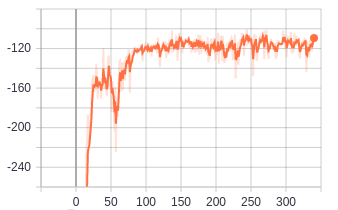
\includegraphics[width=0.5\textwidth]{mountaincar_reward.png}
    \caption{Reward Plot of MountainCar-v0 training}
    \label{fig:mountaincar_reward}
\end{figure}


\begin{table}[H]
\centering
\begin{tabular}{llllll}
\hline
feature & clang  & gcc    & icc    & H      & L      \\ \hline
0       & 300599 & 259228 & 256805 & 453070 & 363562 \\
cmp3    & 53406  & 44174  & 44225  & 76154  & 65651  \\
cwde0   & 22     & 724    & 0      & 37     & 709    \\
dec2    & 573    & 173    & 374    & 802    & 318    \\
leave0  & 3      & 1317   & 5749   & 11     & 7058   \\
movapd3 & 2515   & 130    & 0      & 1969   & 676    \\
movaps2 & 965    & 710    & 4316   & 4777   & 1214   \\
movhps3 & 0      & 8      & 143    & 149    & 2      \\
movlpd3 & 64     & 1594   & 4      & 748    & 914    \\
xorps3  & 18     & 31     & 311    & 284    & 76     \\ \hline
\end{tabular}
\caption{Frequency of tokens over the different classes}
\label{tab:features-frequencies}
\end{table}
\subsection{Pong-v0}


\end{document}


